\begin{enumerate}[label=\thechapter.\arabic*,ref=\thechapter.\theenumi]
\numberwithin{equation}{enumi}
\numberwithin{figure}{enumi}
\numberwithin{table}{enumi}

\item Reduce $x-\sqrt{3}y+8=0$ into normal form. Find its perpendicular distance from the origin and angle between perpendicular and the positive x-axis. 
\\
\solution 
\label{11/10/3/3/1/lagmul}
\iffalse
\documentclass[12pt]{article}
\usepackage{graphicx}
\usepackage[none]{hyphenat}
\usepackage{graphicx}
\usepackage{listings}
\usepackage[english]{babel}
\usepackage{graphicx}
\usepackage{caption} 
\usepackage{booktabs}
\usepackage{array}
\usepackage{amssymb} % for \because
\usepackage{amsmath}   % for having text in math mode
\usepackage{extarrows} % for Row operations arrows
\usepackage{listings}
\lstset{
  frame=single,
  breaklines=true
}
\usepackage{hyperref}
  
%Following 2 lines were added to remove the blank page at the beginning
\usepackage{atbegshi}% http://ctan.org/pkg/atbegshi
\AtBeginDocument{\AtBeginShipoutNext{\AtBeginShipoutDiscard}}
\usepackage{gensymb}


%New macro definitions
\newcommand{\mydet}[1]{\ensuremath{\begin{vmatrix}#1\end{vmatrix}}}
\providecommand{\brak}[1]{\ensuremath{\left(#1\right)}}
\providecommand{\sbrak}[1]{\ensuremath{{}\left[#1\right]}}
\providecommand{\norm}[1]{\left\lVert#1\right\rVert}
\providecommand{\abs}[1]{\left\vert#1\right\vert}
\newcommand{\solution}{\noindent \textbf{Solution: }}
\newcommand{\myvec}[1]{\ensuremath{\begin{pmatrix}#1\end{pmatrix}}}
\let\vec\mathbf


\begin{document}

\begin{center}
\title{\textbf{Lagrange Multipliers}}
\date{\vspace{-5ex}} %Not to print date automatically
\maketitle
\end{center}
\setcounter{page}{1}

\section{11$^{th}$ Maths - Chapter 10}
This is Problem-3.1 from Exercise 10.3 
\begin{enumerate}

\solution 

The equation of the given line is 
\begin{align}
	\myvec{1 \\ -\sqrt{3}}^\top\vec{x}+8 &= 0
\end{align}
Let $\vec{O}$ be the point from where we have to find the perpendicular distance. The perpendicular distance will be the minimum distance from $\vec{O}$ to the line. Let $\vec{P}$ be the foot of the perpendicular. 
\fi
		The given  problem can be formulated as 
\begin{align}
	\label{eq:11/10/3/3/1/lagmul/Eq3}
	\min_{\vec{x}} f\brak{\vec{x}} &= \norm{\vec{x}-\vec{O}}^2\\
	\text{s.t.} \quad g\brak{\vec{x}} = \vec{n}^T\vec{x}-c &= 0 
	\label{eq:11/10/3/3/1/lagmul/Eq1}
\end{align}
where
\begin{align}
	\vec{n} = \myvec{1 \\ -\sqrt{3}},\, 
	\vec{O} = \myvec{0 \\ 0},\,
	\text{ and } c = -8
\end{align}
Define
\begin{align}
	H\brak{\vec{x}, \lambda} &= f\brak{\vec{x}} - \lambda g\brak{\vec{x}} 
\end{align}
and we find that 
\begin{align}
	\nabla f\brak{\vec{x}} &= 2\brak{\vec{x}-\vec{O}} \\
        \nabla g\brak{\vec{x}} &= \vec{n}
\end{align}
We have to find $\lambda \in \mathbb{R}$ such that
\begin{align}
	&\nabla H\brak{\vec{x},\lambda} = 0 \\
        \label{eq:11/10/3/3/1/lagmul/Eqlambda}
	&\implies 2\brak{\vec{x}-\vec{O}} - \lambda\vec{n} = 0 \\
        \label{eq:11/10/3/3/1/lagmul/Eqx}
	&\implies \vec{x} = \frac{\lambda}{2}\vec{n} + \vec{O} 
\end{align}
Substituting \eqref{eq:11/10/3/3/1/lagmul/Eqx} in \eqref{eq:11/10/3/3/1/lagmul/Eq1}
\begin{align}
	\vec{n}^\top\brak{\frac{\lambda}{2}\vec{n} + \vec{O}}-c &= 0 \\
	\implies \lambda &= \frac{2\brak{c-\vec{n}^\top\vec{O}}}{\norm{\vec{n}}^2}
\end{align}
Substituting the value of $\lambda$ in \eqref{eq:11/10/3/3/1/lagmul/Eqlambda}, 
\begin{align}
	\vec{x}_{min} &= \vec{P} = \vec{O}+ \frac{\vec{n}\brak{c-\vec{n}^\top\vec{O}}}{\norm{\vec{n}}^2}\\
	&= \myvec{0 \\0}+ \frac{\myvec{1 \\ -\sqrt{3}}\brak{-8-\myvec{1 & -\sqrt{3}}\myvec{0 \\0}}}{4} \\
	&= \myvec{-2 \\ 2\sqrt{3}} \\
	OP &= \norm{\vec{P}-\vec{O}}^2 \\ 
	&= \norm{\myvec{-2 \\ 2\sqrt{3}}-\myvec{0 \\ 0}} \\
	&=  4
\end{align}	
The relevant figure is shown in \ref{fig:11/10/3/3/1/lagmul/Fig1}
\begin{figure}[!h]
	\begin{center}
		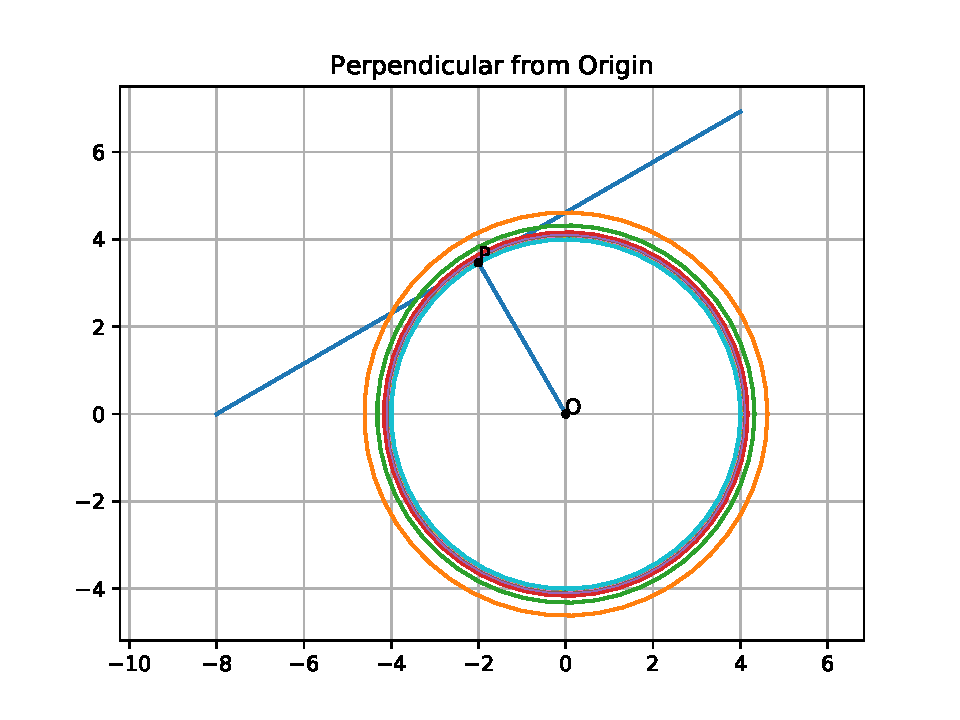
\includegraphics[width=\columnwidth]{11/10/3/3/1/lagmul/figs/problem3.1.pdf}
	\end{center}
\caption{}
\label{fig:11/10/3/3/1/lagmul/Fig1}
\end{figure}

\item Reduce the equation $y-2=0$ into normal form. Find the perpendicular distances from the origin and angle between perpendicular and the positive x-axis.
\\
\solution 
\label{11/10/3/3/2/lagmul}
\iffalse
\documentclass[12pt]{article}
\usepackage{graphicx}
\usepackage{amsmath}
\usepackage{mathtools}
\usepackage{gensymb}
\usepackage{tabularx}
\usepackage{array}
\usepackage[latin1]{inputenc}
\usepackage{fullpage}
\usepackage{color}
\usepackage{array}
\usepackage{longtable}
\usepackage{calc}
\usepackage{multirow}
\usepackage{hhline}
\usepackage{ifthen}
\usepackage{lscape}
\usepackage{float}
\usepackage{amssymb}

\newcommand{\mydet}[1]{\ensuremath{\begin{vmatrix}#1\end{vmatrix}}}
\providecommand{\brak}[1]{\ensuremath{\left(#1\right)}}
\providecommand{\cbrak}[1]{\ensuremath{\left\{#1\right\}}}
\providecommand{\norm}[1]{\left\lVert#1\right\rVert}
\providecommand{\abs}[1]{\left\vert#1\right\vert}
\newcommand{\solution}{\noindent \textbf{Solution: }}
\newcommand{\myvec}[1]{\ensuremath{\begin{pmatrix}#1\end{pmatrix}}}
\let\vec\mathbf

\def\inputGnumericTable{}

\begin{document}
\begin{center}
\textbf\large{OPTIMIZATION}

\end{center}
\section*{Excercise 10.3}

Q.3.2 
\solution
The given equation can be written as
\begin{align}
	\label{eq:11/10/3/3/2/lagmul/eq1}
	\myvec{0&1}\vec{x} &= 2
\end{align}
Let $\vec{O}$ be the point from where we have to find the perpendicular distance. The perpendicular distance will be the minimum distance from $\vec{O}$ to theline. Let $\vec{P}$ be the foot of perpendicular. 
\fi
The given problem can be formulated as 
\begin{align}
	\min_{\vec{x}}f\brak{\vec{x}} &= \norm{\vec{x}-\vec{O}}^2\\
	\text{s.t. } g\brak{\vec{x}} &= \vec{n}^\top\vec{x}-c=0
	\label{eq:11/10/3/3/2/lagmul/eq1}
\end{align}
where
\begin{align}
	\vec{n} = \myvec{0\\1},\,
	\vec{O} = \myvec{0\\0},
	c = 2
\end{align}
Define
\begin{align}
	H\brak{\vec{x},\lambda} = f\brak{\vec{x}} - \lambda g\brak{\vec{x}}
\end{align}
Since
\begin{align}
	\nabla f\brak{\vec{x}} &= 2\brak{\vec{x}-\vec{O}}\\
	\nabla g\brak{\vec{x}} &= \vec{n}
\end{align}
We have to find $\lambda \in \mathbb{R}$ such that
\begin{align}
	\nabla H\brak{\vec{x},\lambda} &= 0\\
	\label{eq:11/10/3/3/2/lagmul/eq2}
	\implies 2\brak{\vec{x}-\vec{O}}-\lambda\vec{n} &= 0\\
	\label{eq:11/10/3/3/2/lagmul/eq3}
	\implies \vec{x} = \frac{\lambda}{2}\vec{n}+\vec{O}
\end{align}
Substituting \eqref{eq:11/10/3/3/2/lagmul/eq3} in \eqref{eq:11/10/3/3/2/lagmul/eq1}
\begin{align}
	\vec{n}^\top\brak{\frac{\lambda}{2}\vec{n}+\vec{O}} - c &= 0\\
	\implies \lambda = \frac{2\brak{c-\vec{n}^\top\vec{O}}}{\norm{\vec{n}}^2} &= 4 > 0
\end{align}
Substituting the value of $\lambda$ in \eqref{eq:11/10/3/3/2/lagmul/eq3},
\begin{align}
	\vec{x}_{min} &=  \vec{O}+\frac{\vec{n}\brak{c-\vec{n}^\top\vec{O}}}{\norm{\vec{n}}^2}
	\\
	&= \myvec{0\\0}+ \frac{\myvec{0\\1}\brak{2-\myvec{0&1}\myvec{0\\0}}}{1}
	= \myvec{0\\2}\\
	\implies OP &= \norm{\vec{P}-\vec{O}}^2
	= 2
\end{align}
See Fig. \ref{fig:11/10/3/3/2/lagmul/Fig1}
\begin{figure}[!h]
	\begin{center} 
	    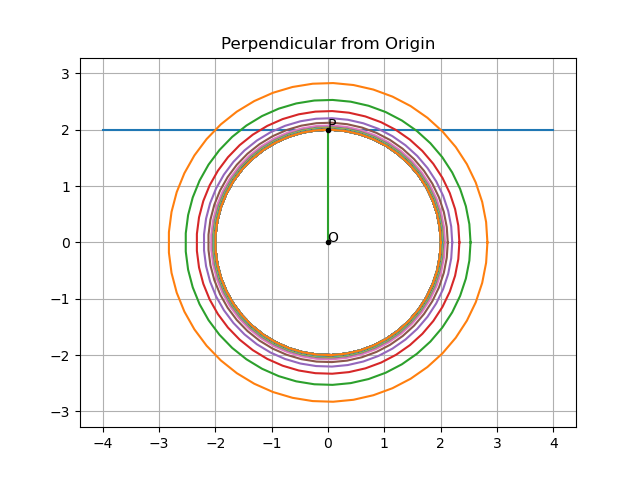
\includegraphics[width=\columnwidth]{11/10/3/3/2/lagmul/figs/opt3}
	\end{center}
\caption{}
\label{fig:11/10/3/3/2/lagmul/Fig1}
\end{figure}

  \item Find the coordinates of the foot of perpendicular from the point 
    \begin{align}
        \vec{P} = \myvec{-1\\3}
        \label{eq:11/10/3/14/lagmul/P-def}
    \end{align}
    to the line 
    \begin{align}
        \myvec{3&-4}\vec{x} = 16
        \label{eq:11/10/3/14/lagmul/line}
    \end{align}
\\
\solution 
\label{11/10/3/14/lagmul}
\iffalse
\documentclass[journal,12pt,twocolumn]{IEEEtran}
\usepackage{setspace}
\usepackage{gensymb}
\singlespacing
\usepackage[cmex10]{amsmath}
\usepackage{amsthm}
\usepackage{mathrsfs}
\usepackage{txfonts}
\usepackage{stfloats}
\usepackage{bm}
\usepackage{cite}
\usepackage{cases}
\usepackage{subfig}
\usepackage{longtable}
\usepackage{multirow}
\usepackage{enumitem}
\usepackage{mathtools}
\usepackage{tikz}
\usepackage{circuitikz}
\usepackage{verbatim}
\usepackage[breaklinks=true]{hyperref}
\usepackage{tkz-euclide} % loads  TikZ and tkz-base
\usepackage{listings}
\usepackage{color}    
\usepackage{array}    
\usepackage{longtable}
\usepackage{calc}     
\usepackage{multirow} 
\usepackage{hhline}   
\usepackage{ifthen}   
\usepackage{lscape}     
\usepackage{chngcntr}
\DeclareMathOperator*{\Res}{Res}
\renewcommand\thesection{\arabic{section}}
\renewcommand\thesubsection{\thesection.\arabic{subsection}}
\renewcommand\thesubsubsection{\thesubsection.\arabic{subsubsection}}

\renewcommand\thesectiondis{\arabic{section}}
\renewcommand\thesubsectiondis{\thesectiondis.\arabic{subsection}}
\renewcommand\thesubsubsectiondis{\thesubsectiondis.\arabic{subsubsection}}
\renewcommand\thetable{\arabic{table}}
% correct bad hyphenation here
\hyphenation{op-tical net-works semi-conduc-tor}
\def\inputGnumericTable{}                                 %%

\lstset{
%language=C,
frame=single, 
breaklines=true,
columns=fullflexible
}
%\lstset{
%language=tex,
%frame=single, 
%breaklines=true
%}

\begin{document}
\newtheorem{theorem}{Theorem}[section]
\newtheorem{problem}{Problem}
\newtheorem{proposition}{Proposition}[section]
\newtheorem{lemma}{Lemma}[section]
\newtheorem{corollary}[theorem]{Corollary}
\newtheorem{example}{Example}[section]
\newtheorem{definition}[problem]{Definition}
\newcommand{\BEQA}{\begin{eqnarray}}
\newcommand{\EEQA}{\end{eqnarray}}
\newcommand{\define}{\stackrel{\triangle}{=}}
\bibliographystyle{IEEEtran}
\providecommand{\mbf}{\mathbf}
\providecommand{\pr}[1]{\ensuremath{\Pr\left(#1\right)}}
\providecommand{\qfunc}[1]{\ensuremath{Q\left(#1\right)}}
\providecommand{\sbrak}[1]{\ensuremath{{}\left[#1\right]}}
\providecommand{\lsbrak}[1]{\ensuremath{{}\left[#1\right.}}
\providecommand{\rsbrak}[1]{\ensuremath{{}\left.#1\right]}}
\providecommand{\brak}[1]{\ensuremath{\left(#1\right)}}
\providecommand{\lbrak}[1]{\ensuremath{\left(#1\right.}}
\providecommand{\rbrak}[1]{\ensuremath{\left.#1\right)}}
\providecommand{\cbrak}[1]{\ensuremath{\left\{#1\right\}}}
\providecommand{\lcbrak}[1]{\ensuremath{\left\{#1\right.}}
\providecommand{\rcbrak}[1]{\ensuremath{\left.#1\right\}}}
\theoremstyle{remark}
\newtheorem{rem}{Remark}
\newcommand{\sgn}{\mathop{\mathrm{sgn}}}
\providecommand{\abs}[1]{\left\vert#1\right\vert}
\providecommand{\res}[1]{\Res\displaylimits_{#1}} 
\providecommand{\norm}[1]{\left\lVert#1\right\rVert}
\providecommand{\mtx}[1]{\mathbf{#1}}
\providecommand{\mean}[1]{E\left[ #1 \right]}
\providecommand{\fourier}{\overset{\mathcal{F}}{ \rightleftharpoons}}
\providecommand{\system}[1]{\overset{\mathcal{#1}}{ \longleftrightarrow}}
\newcommand{\solution}{\noindent \textbf{Solution: }}
\newcommand{\cosec}{\,\text{cosec}\,}
\providecommand{\dec}[2]{\ensuremath{\overset{#1}{\underset{#2}{\gtrless}}}}
\newcommand{\myvec}[1]{\ensuremath{\begin{pmatrix}#1\end{pmatrix}}}
\newcommand{\mydet}[1]{\ensuremath{\begin{vmatrix}#1\end{vmatrix}}}
\let\vec\mathbf
\def\putbox#1#2#3{\makebox[0in][l]{\makebox[#1][l]{}\raisebox{\baselineskip}[0in][0in]{\raisebox{#2}[0in][0in]{#3}}}}
     \def\rightbox#1{\makebox[0in][r]{#1}}
     \def\centbox#1{\makebox[0in]{#1}}
     \def\topbox#1{\raisebox{-\baselineskip}[0in][0in]{#1}}
     \def\midbox#1{\raisebox{-0.5\baselineskip}[0in][0in]{#1}}

\vspace{3cm}
\title{Optimization Assignment}
\author{Gautam Singh}
\maketitle
\bigskip

\begin{abstract}
    This document contains the solution to Question 4 of Exercise 2 in Chapter
    10 of the class 11 NCERT textbook.
\end{abstract}

\begin{enumerate}
  
    \solution 
    \fi
		We rewrite the problem as
    \begin{align}
        \min_{\vec{x}} h\brak{\vec{x}} &\triangleq \norm{\vec{x}-\vec{P}}^2 \\
        \textrm{s.t. } g\brak{\vec{x}} &\triangleq \vec{n}^\top\vec{x} - c = 0
        \label{eq:11/10/3/14/lagmul/lag-opt}
    \end{align}
    where
    \begin{align}
        \vec{P} = \myvec{-1\\3},\ \vec{n} = \myvec{3\\-4},\ c = 16
        \label{eq:11/10/3/14/lagmul/vals}
    \end{align}
    Define
    \begin{align}
        C\brak{\vec{x},\lambda} &= h\brak{\vec{x}} - \lambda g\brak{\vec{x}}
        \label{eq:11/10/3/14/lagmul/C-def}
    \end{align}
    and note that
    \begin{align}
        \nabla h\brak{\vec{x}} &= 2\brak{\vec{x}-\vec{P}} \\
        \nabla g\brak{\vec{x}} &= \vec{n}
        \label{eq:11/10/3/14/lagmul/diff-gh}
    \end{align}
    We are required to find $\lambda \in \mathbb{R}$ such that
    \begin{align}
        \nabla C\brak{\vec{x},\lambda} &= 0 \\
        \implies 2\brak{\vec{x}-\vec{P}} - \lambda\vec{n} &= 0
        \label{eq:11/10/3/14/lagmul/x-lambda}
    \end{align}
    However, $\vec{x}$ lies on the line \eqref{eq:11/10/3/14/lagmul/line}. Thus, from
    \eqref{eq:11/10/3/14/lagmul/x-lambda},
    \begin{align}
        \vec{n}^\top\brak{\frac{\lambda}{2}\vec{n}+\vec{P}} - c &= 0 \\
        \implies \lambda &= \frac{2\brak{c-\vec{n}^\top\vec{P}}}{\norm{\vec{n}}^2}
        \label{eq:11/10/3/14/lagmul/lambda-opt}
    \end{align}
    Substituting \eqref{eq:11/10/3/14/lagmul/lambda-opt} in \eqref{eq:11/10/3/14/lagmul/x-lambda}, the optimal
    point is given by
    \begin{align}
        \vec{Q} &= \vec{P} + \frac{\lambda}{2}\vec{n} \\
                &= \vec{P} - \frac{\vec{n}^\top\vec{P}-c}{\norm{\vec{n}}^2}\vec{n}
                \label{eq:11/10/3/14/lagmul/x-sol-lag}
    \end{align}
    Substituting from \eqref{eq:11/10/3/14/lagmul/vals},
    \begin{align}
        \lambda = \frac{62}{25},\ \vec{Q} = \frac{1}{25}\myvec{68\\-49}
        \label{eq:11/10/3/14/lagmul/sol}
    \end{align}
    To find $\vec{Q}$ graphically, we use constrained gradient descent, with
    learning rate $\alpha = 0.01$. The results are shown in Fig.
    \ref{fig:11/10/3/14/lagmul/gd-lag}, plotted using the Python code.
    \begin{figure}[!ht]
        \centering
        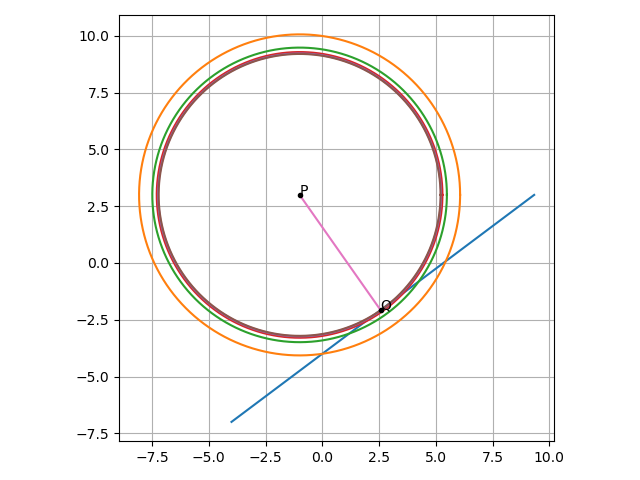
\includegraphics[width=\columnwidth]{11/10/3/14/lagmul/figs/gd_lagrange.png}
        \caption{Constrained gradient descent to find optimal $\vec{Q}$.}
        \label{fig:11/10/3/14/lagmul/gd-lag}
    \end{figure}
\textit{Constrained gradient descent} is a method of optimizing the cost function
subject to some constraints, represented as follows.
\begin{align}
    \max_{\vec{x}}f\brak{\vec{x}} \label{eq:11/10/3/14/lagmul/cgd-cost} \\
    \textrm{s.t. } g\brak{\vec{x}} = 0
    \label{eq:11/10/3/14/lagmul/cgd-constr}
\end{align}
Unlike the unconstrained version, one cannot move in the negative direction of the
gradient vector of $f\brak{\vec{x}}$. However, we must move along the constraint in
\eqref{eq:11/10/3/14/lagmul/cgd-constr}.

The algorithm terminates when the gradient vector of $f$ is parallel to the normal 
vector of $g$ at that point. Mathematically, at an optimum $\vec{x_o}$,
\begin{align}
    \nabla f\brak{\vec{x_o}} = \lambda\nabla g\brak{\vec{x_o}}
    \label{eq:11/10/3/14/lagmul/cgd-cond}
\end{align}
where $\lambda \in \mathbb{R}\setminus\cbrak{0}$. Observe that \eqref{eq:11/10/3/14/lagmul/cgd-cond}
may be rewritten as
\begin{align}
    \nabla C\brak{\vec{x},\lambda} = \nabla \brak{f\brak{\vec{x}}-\lambda g\brak{\vec{x}}} = 0
\end{align}
which is analogous to the method of Lagrangian multipliers.


  \item The point on the curve 
    \begin{align}
        x^2 = 2y
        \label{eq:12/6/5/27/nonconv/lagmul/curve}
    \end{align}
    which is nearest to the point 
    $\vec{P} = \myvec{0\\5}$ is
    \begin{enumerate}
        \item $\myvec{2\sqrt{2}\\4}$
        \item $\myvec{2\sqrt{2}\\0}$
        \item $\myvec{0\\0}$
        \item $\myvec{2\\2}$
    \end{enumerate}
\solution 
\label{12/6/5/27/nonconv/lagmul}
\iffalse
\documentclass[journal,12pt,twocolumn]{IEEEtran}
\usepackage{setspace}
\usepackage{gensymb}
\usepackage{xcolor}
\usepackage{caption}
\singlespacing
\usepackage{siunitx}
\usepackage[cmex10]{amsmath}
\usepackage{mathtools}
\usepackage{hyperref}
\usepackage{amsthm}
\usepackage{mathrsfs}
\usepackage{txfonts}
\usepackage{stfloats}
\usepackage{cite}
\usepackage{cases}
\usepackage{subfig}
\usepackage{longtable}
\usepackage{multirow}
\usepackage{enumitem}
\usepackage{bm}
\usepackage{mathtools}
\usepackage{listings}
\usepackage{tikz}
\usetikzlibrary{shapes,arrows,positioning}
\usepackage{circuitikz}
\renewcommand{\vec}[1]{\boldsymbol{\mathbf{#1}}}
\DeclareMathOperator*{\Res}{Res}
\renewcommand\thesection{\arabic{section}}
\renewcommand\thesubsection{\thesection.\arabic{subsection}}
\renewcommand\thesubsubsection{\thesubsection.\arabic{subsubsection}}

\renewcommand\thesectiondis{\arabic{section}}
\renewcommand\thesubsectiondis{\thesectiondis.\arabic{subsection}}
\renewcommand\thesubsubsectiondis{\thesubsectiondis.\arabic{subsubsection}}
\hyphenation{op-tical net-works semi-conduc-tor}

\lstset{
language=Python,
frame=single, 
breaklines=true,
columns=fullflexible
}
\begin{document}
\theoremstyle{definition}
\newtheorem{theorem}{Theorem}[section]
\newtheorem{problem}{Problem}
\newtheorem{proposition}{Proposition}[section]
\newtheorem{lemma}{Lemma}[section]
\newtheorem{corollary}[theorem]{Corollary}
\newtheorem{example}{Example}[section]
\newtheorem{definition}{Definition}[section]
\newcommand{\BEQA}{\begin{eqnarray}}
\newcommand{\EEQA}{\end{eqnarray}}
\newcommand{\define}{\stackrel{\triangle}{=}}
\newcommand{\myvec}[1]{\ensuremath{\begin{pmatrix}#1\end{pmatrix}}}
\newcommand{\mydet}[1]{\ensuremath{\begin{vmatrix}#1\end{vmatrix}}}
\bibliographystyle{IEEEtran}
\providecommand{\nCr}[2]{\,^{#1}C_{#2}} % nCr
\providecommand{\nPr}[2]{\,^{#1}P_{#2}} % nPr
\providecommand{\mbf}{\mathbf}
\providecommand{\pr}[1]{\ensuremath{\Pr\left(#1\right)}}
\providecommand{\qfunc}[1]{\ensuremath{Q\left(#1\right)}}
\providecommand{\sbrak}[1]{\ensuremath{{}\left[#1\right]}}
\providecommand{\lsbrak}[1]{\ensuremath{{}\left[#1\right.}}
\providecommand{\rsbrak}[1]{\ensuremath{{}\left.#1\right]}}
\providecommand{\brak}[1]{\ensuremath{\left(#1\right)}}
\providecommand{\lbrak}[1]{\ensuremath{\left(#1\right.}}
\providecommand{\rbrak}[1]{\ensuremath{\left.#1\right)}}
\providecommand{\cbrak}[1]{\ensuremath{\left\{#1\right\}}}
\providecommand{\lcbrak}[1]{\ensuremath{\left\{#1\right.}}
\providecommand{\rcbrak}[1]{\ensuremath{\left.#1\right\}}}
\theoremstyle{remark}
\newtheorem{rem}{Remark}
\newcommand{\sgn}{\mathop{\mathrm{sgn}}}
\newcommand{\rect}{\mathop{\mathrm{rect}}}
\newcommand{\sinc}{\mathop{\mathrm{sinc}}}
\providecommand{\abs}[1]{\left\vert#1\right\vert}
\providecommand{\res}[1]{\Res\displaylimits_{#1}} 
\providecommand{\norm}[1]{\left\Vert#1\right\Vert}
\providecommand{\mtx}[1]{\mathbf{#1}}
\providecommand{\mean}[1]{E\left[ #1 \right]}
\providecommand{\fourier}{\overset{\mathcal{F}}{ \rightleftharpoons}}
\providecommand{\ztrans}{\overset{\mathcal{Z}}{ \rightleftharpoons}}
\providecommand{\system}[1]{\overset{\mathcal{#1}}{ \longleftrightarrow}}
\newcommand{\solution}{\noindent \textbf{Solution: }}
\providecommand{\dec}[2]{\ensuremath{\overset{#1}{\underset{#2}{\gtrless}}}}
\let\StandardTheFigure\thefigure
\def\putbox#1#2#3{\makebox[0in][l]{\makebox[#1][l]{}\raisebox{\baselineskip}[0in][0in]{\raisebox{#2}[0in][0in]{#3}}}}
     \def\rightbox#1{\makebox[0in][r]{#1}}
     \def\centbox#1{\makebox[0in]{#1}}
     \def\topbox#1{\raisebox{-\baselineskip}[0in][0in]{#1}}
     \def\midbox#1{\raisebox{-0.5\baselineskip}[0in][0in]{#1}}

\vspace{3cm}
\title{Quadratic Programming Assignment}
\author{Gautam Singh}
\maketitle
\bigskip

\begin{abstract}
    This document contains the solution to Question 27 of Exercise 5 in Chapter
    6 of the class 12 NCERT textbook.
\end{abstract}

\begin{enumerate}
  
    \solution 
    \fi
		We need to find
    \begin{align}
        \min_{\vec{x}} g\brak{\vec{x}} &= \norm{\vec{x}-\vec{P}}^2 \label{eq:12/6/5/27/nonconv/lagmul/cost} \\
        \textrm{s.t. } h\brak{\vec{x}} &= \vec{x}^\top\vec{Vx} + 2\vec{u}^\top\vec{x} = 0 \label{eq:12/6/5/27/nonconv/lagmul/constr}
    \end{align}
    where
    \begin{align}
        \vec{V} = \myvec{1&0\\0&0},\ \vec{u} = \myvec{0\\-1}
    \end{align}

    Since the given optimization problem is nonconvex, we use the method of 
    Lagrange multipliers to find the optima. Here, we need to find 
    $\lambda \in \mathbb{R}$ such that there exists a $\vec{x}$ 
    satisfying
    \begin{align}
        \nabla g\brak{\vec{x}} &= \lambda\nabla h\brak{\vec{x}} \\
        \implies 2\brak{\vec{x}-\vec{P}} &= 2\lambda\brak{\vec{Ax}+\vec{u}} \\
        \implies \brak{\vec{I}-\lambda\vec{A}}\vec{x} &= \lambda\vec{u} + \vec{P} \\
        \implies \myvec{1-\lambda&0\\0&1}\vec{x} &= \myvec{0\\5-\lambda}
        \label{eq:12/6/5/27/nonconv/lagmul/lagmul}
    \end{align}
    From \eqref{eq:12/6/5/27/nonconv/lagmul/lagmul}, we have two cases:
    \begin{enumerate}
        \item $\lambda \neq 1$. In this case, we form the augmented matrix
        \begin{align}
            \myvec{1-\lambda&0&0\\0&1&5-\lambda} \xleftrightarrow[]{R_1 \leftarrow \frac{R_1}{1-\lambda}} \myvec{1&0&0\\0&1&5-\lambda}
        \end{align}
        and get that
        \begin{align}
            \vec{x_m} = \myvec{0\\5-\lambda}
        \end{align}
        Substituting in \eqref{eq:12/6/5/27/nonconv/lagmul/constr} gives $\lambda = 5$. Thus, 
        $\vec{x_m} = \vec{0}$.

        \item $\lambda = 1$. In this case, \eqref{eq:12/6/5/27/nonconv/lagmul/lagmul} becomes
        \begin{align}
            \myvec{0&0\\0&1}\vec{x} &= \myvec{0\\4} \\
            \implies \vec{e_2}^\top\vec{x} = 4
            \label{eq:12/6/5/27/nonconv/lagmul/x-e2}
        \end{align}
        Substituting \eqref{eq:12/6/5/27/nonconv/lagmul/x-e2} into \eqref{eq:12/6/5/27/nonconv/lagmul/constr} becomes
        \begin{align}
            \brak{\vec{e_1}^\top\vec{x}}^2 &= 8 \\
            \implies \vec{e_1}^\top\vec{x} &= \pm 2\sqrt{2}
            \label{eq:12/6/5/27/nonconv/lagmul/x-e1}
        \end{align}
        Using \eqref{eq:12/6/5/27/nonconv/lagmul/x-e1} and \eqref{eq:12/6/5/27/nonconv/lagmul/x-e2},
        \begin{align}
            \vec{x_m} = \myvec{\pm 2\sqrt{2}\\4}
        \end{align}
    \end{enumerate}
    Using these values of $\vec{x_m}$, the distances are
    \begin{align}
        \norm{\myvec{0\\5}-\myvec{0\\0}} &= 5 \\
        \norm{\myvec{0\\5}-\myvec{\pm 2\sqrt{2}\\4}} &= 3
        \label{eq:12/6/5/27/nonconv/lagmul/true-min}
    \end{align}
    Thus, the correct answer is \textbf{a)}.

 \item Find the point on the curve 
    \begin{align}
        x^2 = 2y
        \label{eq:curve}
    \end{align}
    which is nearest to the point $\vec{P} = \myvec{2\\1}$.
    \\
\solution 
\label{12/6/5/27/conv/lagmul}
\iffalse
\documentclass[journal,12pt,twocolumn]{IEEEtran}
\usepackage{setspace}
\usepackage{gensymb}
\usepackage{xcolor}
\usepackage{caption}
\singlespacing
\usepackage{siunitx}
\usepackage[cmex10]{amsmath}
\usepackage{mathtools}
\usepackage{hyperref}
\usepackage{amsthm}
\usepackage{mathrsfs}
\usepackage{txfonts}
\usepackage{stfloats}
\usepackage{cite}
\usepackage{cases}
\usepackage{subfig}
\usepackage{longtable}
\usepackage{multirow}
\usepackage{enumitem}
\usepackage{bm}
\usepackage{mathtools}
\usepackage{listings}
\usepackage{tikz}
\usetikzlibrary{shapes,arrows,positioning}
\usepackage{circuitikz}
\renewcommand{\vec}[1]{\boldsymbol{\mathbf{#1}}}
\DeclareMathOperator*{\Res}{Res}
\renewcommand\thesection{\arabic{section}}
\renewcommand\thesubsection{\thesection.\arabic{subsection}}
\renewcommand\thesubsubsection{\thesubsection.\arabic{subsubsection}}

\renewcommand\thesectiondis{\arabic{section}}
\renewcommand\thesubsectiondis{\thesectiondis.\arabic{subsection}}
\renewcommand\thesubsubsectiondis{\thesubsectiondis.\arabic{subsubsection}}
\hyphenation{op-tical net-works semi-conduc-tor}

\lstset{
language=Python,
frame=single, 
breaklines=true,
columns=fullflexible
}
\begin{document}
\theoremstyle{definition}
\newtheorem{theorem}{Theorem}[section]
\newtheorem{problem}{Problem}
\newtheorem{proposition}{Proposition}[section]
\newtheorem{lemma}{Lemma}[section]
\newtheorem{corollary}[theorem]{Corollary}
\newtheorem{example}{Example}[section]
\newtheorem{definition}{Definition}[section]
\newcommand{\BEQA}{\begin{eqnarray}}
\newcommand{\EEQA}{\end{eqnarray}}
\newcommand{\define}{\stackrel{\triangle}{=}}
\newcommand{\myvec}[1]{\ensuremath{\begin{pmatrix}#1\end{pmatrix}}}
\newcommand{\mydet}[1]{\ensuremath{\begin{vmatrix}#1\end{vmatrix}}}
\bibliographystyle{IEEEtran}
\providecommand{\nCr}[2]{\,^{#1}C_{#2}} % nCr
\providecommand{\nPr}[2]{\,^{#1}P_{#2}} % nPr
\providecommand{\mbf}{\mathbf}
\providecommand{\pr}[1]{\ensuremath{\Pr\left(#1\right)}}
\providecommand{\qfunc}[1]{\ensuremath{Q\left(#1\right)}}
\providecommand{\sbrak}[1]{\ensuremath{{}\left[#1\right]}}
\providecommand{\lsbrak}[1]{\ensuremath{{}\left[#1\right.}}
\providecommand{\rsbrak}[1]{\ensuremath{{}\left.#1\right]}}
\providecommand{\brak}[1]{\ensuremath{\left(#1\right)}}
\providecommand{\lbrak}[1]{\ensuremath{\left(#1\right.}}
\providecommand{\rbrak}[1]{\ensuremath{\left.#1\right)}}
\providecommand{\cbrak}[1]{\ensuremath{\left\{#1\right\}}}
\providecommand{\lcbrak}[1]{\ensuremath{\left\{#1\right.}}
\providecommand{\rcbrak}[1]{\ensuremath{\left.#1\right\}}}
\theoremstyle{remark}
\newtheorem{rem}{Remark}
\newcommand{\sgn}{\mathop{\mathrm{sgn}}}
\newcommand{\rect}{\mathop{\mathrm{rect}}}
\newcommand{\sinc}{\mathop{\mathrm{sinc}}}
\providecommand{\abs}[1]{\left\vert#1\right\vert}
\providecommand{\res}[1]{\Res\displaylimits_{#1}} 
\providecommand{\norm}[1]{\left\Vert#1\right\Vert}
\providecommand{\mtx}[1]{\mathbf{#1}}
\providecommand{\mean}[1]{E\left[ #1 \right]}
\providecommand{\fourier}{\overset{\mathcal{F}}{ \rightleftharpoons}}
\providecommand{\ztrans}{\overset{\mathcal{Z}}{ \rightleftharpoons}}
\providecommand{\system}[1]{\overset{\mathcal{#1}}{ \longleftrightarrow}}
\newcommand{\solution}{\noindent \textbf{Solution: }}
\providecommand{\dec}[2]{\ensuremath{\overset{#1}{\underset{#2}{\gtrless}}}}
\let\StandardTheFigure\thefigure
\def\putbox#1#2#3{\makebox[0in][l]{\makebox[#1][l]{}\raisebox{\baselineskip}[0in][0in]{\raisebox{#2}[0in][0in]{#3}}}}
     \def\rightbox#1{\makebox[0in][r]{#1}}
     \def\centbox#1{\makebox[0in]{#1}}
     \def\topbox#1{\raisebox{-\baselineskip}[0in][0in]{#1}}
     \def\midbox#1{\raisebox{-0.5\baselineskip}[0in][0in]{#1}}

\vspace{3cm}
\title{Quadratic Programming Assignment}
\author{Gautam Singh}
\maketitle
\bigskip

\begin{abstract}
    This document contains the solution to a modification of Question 27 of 
    Exercise 5 in Chapter 6 of the class 12 NCERT textbook.
\end{abstract}

\begin{enumerate}
   
    \solution 
\fi
		We need to find
    \begin{align}
        \min_{\vec{x}} g\brak{\vec{x}} &= \norm{\vec{x}-\vec{P}}^2 \label{eq:12/6/5/27/conv/lagmulcost} \\
        \textrm{s.t. } h\brak{\vec{x}} &= \vec{x}^\top\vec{Vx} + 2\vec{u}^\top\vec{x} = 0 \label{eq:12/6/5/27/conv/lagmulconstr}
    \end{align}
    where
    \begin{align}
        \vec{V} = \myvec{1&0\\0&0},\ \vec{u} = \myvec{0\\-1}
    \end{align}

    We use the method of Lagrange multipliers to find the optima. Here, we need 
    to find $\lambda \in \mathbb{R}$ such that there exists a $\vec{x}$ 
    satisfying
    \begin{align}
        \nabla g\brak{\vec{x}} &= \lambda\nabla h\brak{\vec{x}} \\
        \implies 2\brak{\vec{x}-\vec{P}} &= 2\lambda\brak{\vec{Vx}+\vec{u}} \\
        \implies \brak{\vec{I}-\lambda\vec{V}}\vec{x} &= \lambda\vec{u} + \vec{P} \\
        \implies \myvec{1-\lambda&0\\0&1}\vec{x} &= \myvec{2\\1-\lambda}
        \label{eq:12/6/5/27/conv/lagmullagmul}
    \end{align}
    From \eqref{eq:12/6/5/27/conv/lagmullagmul}, we have two cases:
    \begin{enumerate}
        \item $\lambda \neq 1$. In this case, we form the augmented matrix
        \begin{align}
            \myvec{1-\lambda&0&2\\0&1&1-\lambda} \xleftrightarrow[]{R_1 \leftarrow \frac{R_1}{1-\lambda}} \myvec{1&0&\frac{2}{1-\lambda}\\0&1&1-\lambda}
        \end{align}
        and get that
        \begin{align}
            \vec{x_m} = \myvec{\frac{2}{1-\lambda}\\1-\lambda}
        \end{align}
        Substituting in \eqref{eq:12/6/5/27/conv/lagmulconstr} with equality gives 
        $\lambda = 1 - 2^{\frac{1}{3}}$. Thus, 
        \begin{align}
            \vec{x_m} = \myvec{2^{\frac{2}{3}}\\2^{\frac{1}{3}}}
        \end{align}

        \item $\lambda = 1$. In this case, \eqref{eq:12/6/5/27/conv/lagmullagmul} becomes
        \begin{align}
            \myvec{0&0\\0&1}\vec{x} &= \myvec{2\\0}
        \end{align}
        which clearly has no solution.
    \end{enumerate}
    Thus, the required point is
    \begin{align}
        \vec{x_m} = \myvec{2^{\frac{2}{3}}\\2^{\frac{1}{3}}}
    \end{align}




\end{enumerate}
